
% Copyright (c) 2015 - 2020 Mario Mlačak, mmlacak@gmail.com
% Licensed and published as Public Domain work.

% Discovery chapter ===================================================
\chapter*{Discovery}
\addcontentsline{toc}{chapter}{Discovery}

\begin{flushright}
\parbox{0.8\textwidth}{
\emph{I don’t believe in God but I’m very interested in her. \\
\hspace*{\fill}{\textperiodcentered \textperiodcentered \textperiodcentered \hspace*{0.2em} Arthur C. Clarke} } }
\end{flushright}

\noindent
Discovery is chess variant which is played on 24 x 24 board, with
light (pastel!) yellow and gray fields and darker gray and dark teal
pieces. Star colors are bright orange and dark violet. In algebraic
notation, columns are enumerated from 'a' to 'x', and rows are
enumerated from '1' to '24'. A new piece is introduced, Monolith.

\clearpage % ..........................................................
% Monolith ************************************************************

\section*{Monolith}
\addcontentsline{toc}{section}{Monolith}

\vspace*{-1.1\baselineskip}
\noindent
\begin{wrapfigure}[11]{l}{0.4\textwidth}
\centering
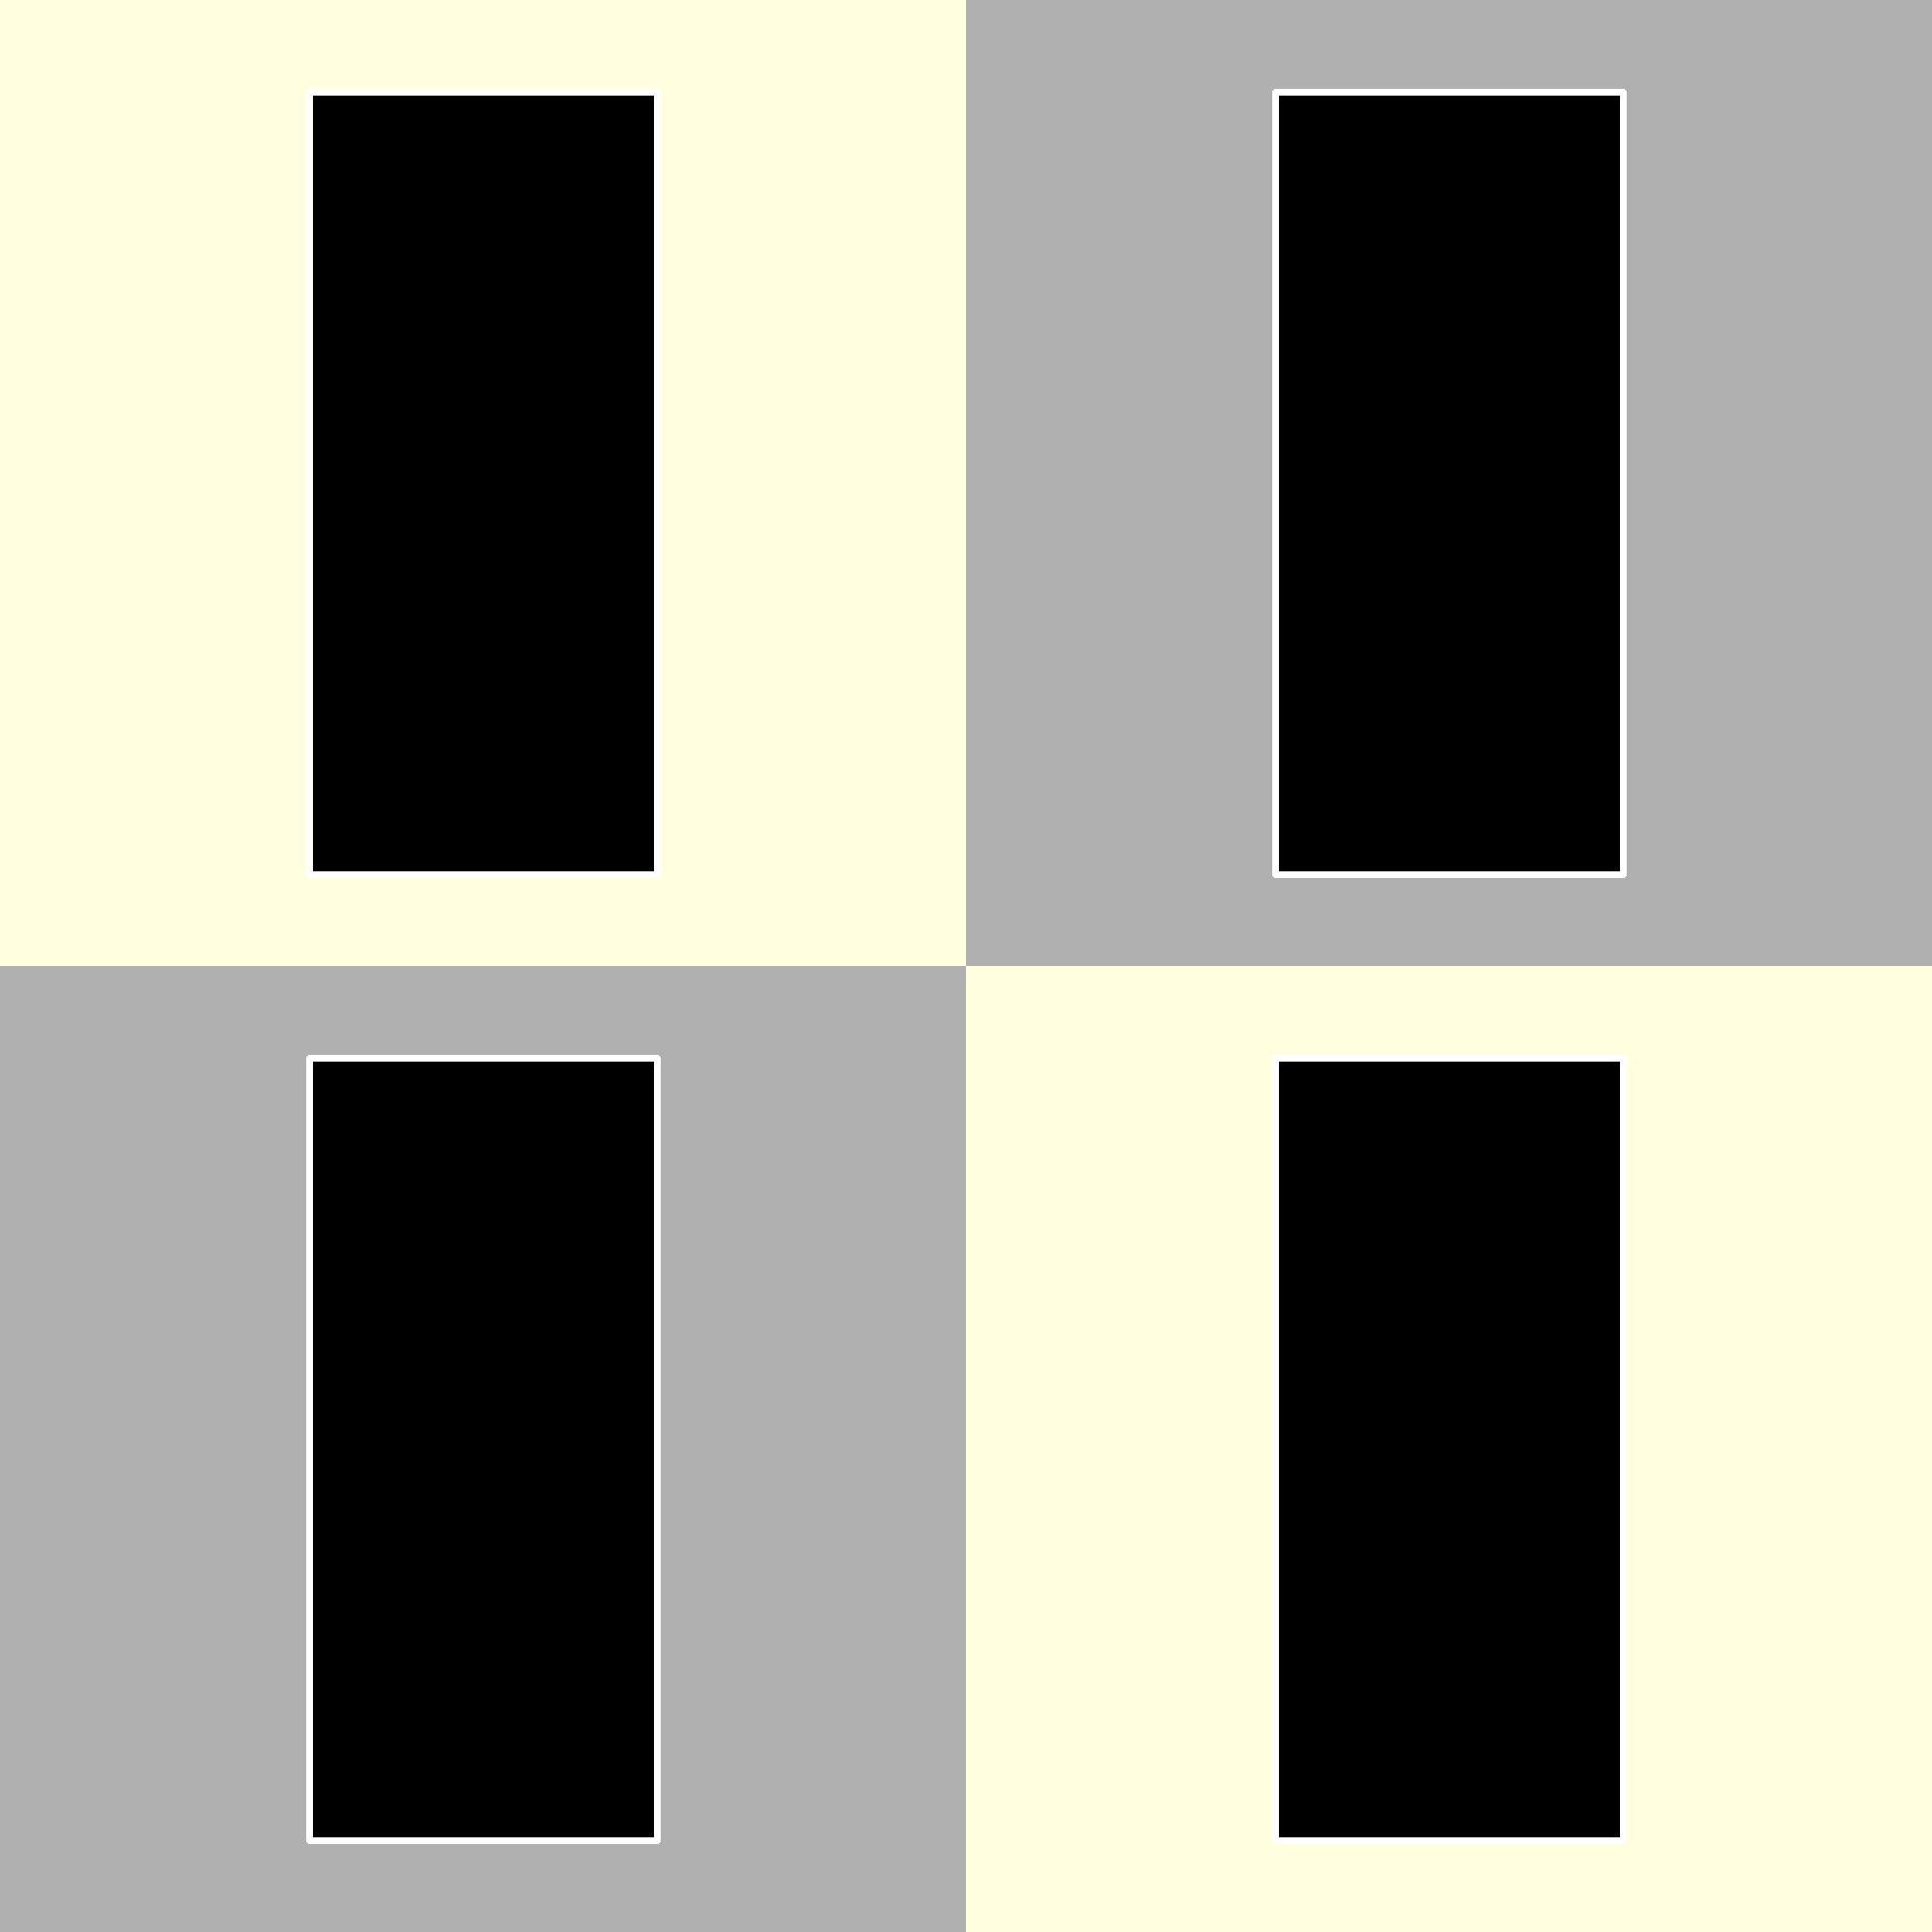
\includegraphics[width=0.4\textwidth, keepaspectratio=true]{pieces/15_monolith.png}
\caption{Monolith}
\label{fig:15_monolith}
\end{wrapfigure}
Monolith does not belong to any player, but can be moved by both of them.
Monolith cannot be captured, converted, nor activated.
Pawns cannot be promoted to Monolith.

Monolith is a teleportation device, much like moveable Star. Piece can
initiate teleportation either by touching a Monolith or a field at which
it stands.

Piece, if not Wave, then reappears on a chosen empty portal-field around
any Star or the other Monolith. Wave teleported from a Monolith can emerge
only from the other Monolith. Kings cannot be teleported.

Piece teleported from a Star, if not Wave, can reappear on a chosen empty
portal-field around the 2 Stars in opposite color, or around any Monolith.
Wave teleported from a Star can only emerge from the Star in the same color.

Monolith cannot capture piece, and thus cannot check, nor checkmate opponent's
King. Monolith cannot activate Wave, nor any other piece.

Monolith moves similar to Knight, but can perform 3 steps in a single ply,
by alternating between left and right steps. All step-fields in a ply must
be empty.

Alternative move for Monolith is syzygy.

In algebraic notation, symbol for Monolith is 'M'.

% \clearpage % ..........................................................

% \vspace*{0.05\textheight}
\noindent
\begin{wrapfigure}[2]{l}{0.4\textwidth}
\centering
\includegraphics[width=0.4\textwidth, keepaspectratio=true]{pieces/bishop/20_discovery.png}
\caption{Bishop}
\label{fig:bishop/20_discovery}
\end{wrapfigure}
Piece colors in this variant are presented on the left.

\vspace*{0.30\textheight}
\noindent
\begin{wrapfigure}[2]{l}{0.4\textwidth}
\centering
\includegraphics[width=0.4\textwidth, keepaspectratio=true]{pieces/star/20_discovery.png}
\caption{Star}
\label{fig:star/20_discovery}
\end{wrapfigure}
Star colors in this variant are presented on the left.

\clearpage % ..........................................................
% Movement ------------------------------------------------------------

\subsection*{Movement}
\addcontentsline{toc}{subsection}{Movement}

\vspace*{-0.3\baselineskip}
\noindent
\begin{wrapfigure}[4]{l}{0.35\textwidth}
\centering
\includegraphics[width=0.291666667\textwidth, keepaspectratio=true]{examples/20_d/scn_d_01_knight_steps.png}
\caption{Knight steps}
\label{fig:scn_d_01_knight_steps}
\end{wrapfigure}
Like in a \hyperref[fig:scn_cot_10_knight_directions]{Conquest of Tlalocan variant},
looking from Knight's position forward, one direction
would be to the left, and the other to the right.

% \vspace*{0.2\textheight}
\vspace*{6.1\baselineskip}
\noindent
\begin{wrapfigure}[9]{l}{0.35\textwidth}
\centering
\includegraphics[width=0.291666667\textwidth, keepaspectratio=true]{examples/20_d/scn_d_02_monolith_steps.png}
\caption{Monolith steps}
\label{fig:scn_d_02_monolith_steps}
\end{wrapfigure}
Here, all left (green) and right (blue) steps of Monolith are marked.

Monolith can freely choose any step-field as its' first step destination. On all
subsequent steps, Monolith has to alternate between left and right steps. Every
step direction can be chosen independently of any previous choice.

% \vspace*{6.1\baselineskip}
\noindent
\begin{wrapfigure}[9]{l}{0.35\textwidth}
\centering
\includegraphics[width=0.291666667\textwidth, keepaspectratio=true]{examples/20_d/scn_d_03_monolith_step_1.png}
\caption{Monolith first step}
\label{fig:scn_d_03_monolith_step_1}
\end{wrapfigure}
Like Knight, Monolith is not obstructed by any piece on unmarked (i.e. non-step)
field. Monolith cannot interact with other pieces on its' own. So, Monolith is
blocked by any piece, except Star or other Monolith, on its' step-field. In this
variant, Monolith is limited to 3 steps in its' ply.

\clearpage % ..........................................................

\noindent
\begin{figure}[!h]
% \begin{figure}[!t]
\includegraphics[width=1.0\textwidth, keepaspectratio=true]{examples/20_d/scn_d_04_monolith_step_2.png}
\caption{Monolith step 2}
\label{fig:scn_d_04_monolith_step_2}
% \centering
\end{figure}

Starting field is marked S. Right step was chosen as a first one, so next step
has to be to the left. Here, Monolith is obstructed by Wave on a step-field.
This is so regardless if player moving Monolith is light or dark.

\clearpage % ..........................................................

\noindent
\begin{figure}[!h]
% \begin{figure}[!t]
\includegraphics[width=1.0\textwidth, keepaspectratio=true]{examples/20_d/scn_d_05_monolith_step_3.png}
\caption{Monolith step 3}
\label{fig:scn_d_05_monolith_step_3}
% \centering
\end{figure}

Previous step was a left one, so next step needs to be one of 4 marked right
steps. This is also last step in a Monolith's ply, since it's third. Monolith
is not obstructed by Pawns on a non-step fields; nor by Bishop on a step-field
in alternate direction (here, left).

% ------------------------------------------------------------ Movement
\clearpage % ..........................................................
% Teleporting ---------------------------------------------------------

\subsection*{Teleporting}
\addcontentsline{toc}{subsection}{Teleporting}

\vspace*{-0.9\baselineskip}
\noindent
\begin{figure}[!h]
% \begin{figure}[!t]
\includegraphics[width=1.0\textwidth, keepaspectratio=true]{examples/20_d/scn_d_06_teleport_via_monolith.png}
\caption{Teleporting piece via Monolith}
\label{fig:scn_d_06_teleport_via_monolith}
% \centering
\end{figure}

Teleportation using Monoliths is similar to one using Stars in \hyperref[fig:scn_n_02_teleport_init]{previous variant, Nineteen}.
Pieces, if not Waves, teleporting from Monolith can reappear near any Star or the other Monolith.
All momentum carried is lost. Again, Kings cannot teleport.
Here, all empty portal-fields where Bishop can be teleported to are enumerated.

\clearpage % ..........................................................

\noindent
\begin{figure}[!h]
% \begin{figure}[!t]
\includegraphics[width=1.0\textwidth, keepaspectratio=true]{examples/20_d/scn_d_07_teleport_via_star.png}
\caption{Teleporting piece via Star}
\label{fig:scn_d_07_teleport_via_star}
% \centering
\end{figure}

All pieces, except Waves, teleporting from a Star can reappear on a empty portal-field
near Stars in opposite color, or near any Monolith.
Here, all empty portal-fields where Bishop can be teleported to are enumerated.

\clearpage % ..........................................................
% Teleporting Wave ....................................................

\subsubsection*{Wave}
\addcontentsline{toc}{subsubsection}{Wave}

\noindent
\begin{figure}[!h]
% \begin{figure}[!t]
\includegraphics[width=1.0\textwidth, keepaspectratio=true]{examples/20_d/scn_d_08_teleport_wave_via_star.png}
\caption{Teleporting Wave via Star}
\label{fig:scn_d_08_teleport_wave_via_star}
% \centering
\end{figure}

...

\clearpage % ..........................................................

\noindent
\begin{figure}[!h]
% \begin{figure}[!t]
\includegraphics[width=1.0\textwidth, keepaspectratio=true]{examples/20_d/scn_d_09_teleport_wave_via_monolith.png}
\caption{Teleporting Wave via Monolith}
\label{fig:scn_d_09_teleport_wave_via_monolith}
% \centering
\end{figure}

...

\clearpage % ..........................................................

\noindent
\begin{figure}[!h]
% \begin{figure}[!t]
\includegraphics[width=1.0\textwidth, keepaspectratio=true]{examples/20_d/scn_d_10_teleported_wave_blocked.png}
\caption{Teleported Wave blocked}
\label{fig:scn_d_10_teleported_wave_blocked}
% \centering
\end{figure}

...

\clearpage % ..........................................................

\noindent
\begin{figure}[!h]
% \begin{figure}[!t]
\includegraphics[width=1.0\textwidth, keepaspectratio=true]{examples/20_d/scn_d_11_wave_teleported_off_board.png}
\caption{Wave teleported off-board}
\label{fig:scn_d_11_wave_teleported_off_board}
% \centering
\end{figure}

...

\clearpage % ..........................................................

\noindent
\begin{figure}[!h]
% \begin{figure}[!t]
\includegraphics[width=1.0\textwidth, keepaspectratio=true]{examples/20_d/scn_d_12_wave_teleport_on_and_off_board.png}
\caption{Teleporting Wave on- and off-board}
\label{fig:scn_d_12_wave_teleport_on_and_off_board}
% \centering
\end{figure}

...

% .................................................... Teleporting Wave
\clearpage % ..........................................................

\subsubsection*{Monolith}
\addcontentsline{toc}{subsubsection}{Monolith}

\noindent
\begin{figure}[!h]
% \begin{figure}[!t]
\includegraphics[width=1.0\textwidth, keepaspectratio=true]{examples/20_d/scn_d_13_teleporting_monolith_via_star.png}
\caption{Teleporting Monolith via Star}
\label{fig:scn_d_13_teleporting_monolith_via_star}
% \centering
\end{figure}

...

\clearpage % ..........................................................

\noindent
\begin{figure}[!h]
% \begin{figure}[!t]
\includegraphics[width=1.0\textwidth, keepaspectratio=true]{examples/20_d/scn_d_14_teleporting_monolith_via_monolith.png}
\caption{Teleporting Monolith via Monolith}
\label{fig:scn_d_14_teleporting_monolith_via_monolith}
% \centering
\end{figure}

...

\clearpage % ..........................................................

\subsubsection*{Shaman's trance-journey}
\addcontentsline{toc}{subsubsection}{Shaman's trance-journey}

\huge{TODO :: Shaman's trance-journey interaction}
\normalsize{}
...

% --------------------------------------------------------- Teleporting
\clearpage % ..........................................................
% Syzygy --------------------------------------------------------------

\subsection*{Syzygy}
\addcontentsline{toc}{subsection}{Syzygy}
...

% -------------------------------------------------------------- Syzygy
% ************************************************************ Monolith
\clearpage % ..........................................................

\section*{Promotion}
\addcontentsline{toc}{section}{Promotion}

Promotion is non enforced, delayed variety, i.e. it's the same as in
\hyperref[sec:Age of Aquarius/Promotion]{previous chess variant}, Age of Aquarius.

Promotion in this variant is polygamous, more than one Queen in the same color
can be present on chessboard at any given time.

Again, Pawn cannot be promoted to Monolith.

\clearpage % ..........................................................

\section*{En passant}
\addcontentsline{toc}{section}{En passant}

\noindent
\begin{wrapfigure}{l}{0.4\textwidth}
\centering

\includegraphics[width=0.125\textwidth, keepaspectratio=true]{en_passants/20_discovery_en_passant.png}
\caption{En passant}
\label{fig:20_discovery_en_passant}
\end{wrapfigure}
Rush and en passant are identical to those in Classic Chess, only difference
is that Pawn can now move longer on initial turn, up to 10 fields in this
variant.

\clearpage % ..........................................................

\section*{Castling}
\addcontentsline{toc}{section}{Castling}

Castling is the same as in Classical Chess, only difference is that King can move between 2 and 9 fields across.
All other constraints from Classical Chess still applies.

\noindent
\begin{figure}[!h]
% \begin{figure}[!t]
\includegraphics[width=1.0\textwidth, keepaspectratio=true]{castlings/20_d/discovery_castling.png}
\caption{Castling}
\label{fig:discovery_castling}
% \centering
\end{figure}

In example above, all valid King's castling moves are numbered.

\noindent
\begin{figure}[!h]
% \begin{figure}[!t]
\includegraphics[width=1.0\textwidth, keepaspectratio=true]{castlings/20_d/discovery_castling_left_07.png}
\caption{Castling long left}
\label{fig:discovery_castling_left_07}
% \centering
\end{figure}

In this example King was castling long to the left. Initial King's position is marked with "K".
After castling is finished, left Rook ends up at field immediately right to the King.

\clearpage % ..........................................................

\section*{Initial setup}
\addcontentsline{toc}{section}{Initial setup}

Compared to initial setup of Conquest of Tlalocan, just 2 Monoliths are placed in to the open,
symetrically, on both sides of chessboard. This can be seen in the image below:

\noindent
% \begin{figure}[t]
\begin{figure}[h]
\includegraphics[width=1.0\textwidth, keepaspectratio=true]{boards/20_discovery.png}
\caption{Discovery board}
\label{fig:20_discovery}
% \centering
\end{figure}

\clearpage % ..........................................................
% =================================================== Discovery chapter
